	% **************************************************************************************************************
% A Classic Thesis Style
% An Homage to The Elements of Typographic Style
%
% Copyright (C) 2011 Andr\'e Miede http://www.miede.de
%
% If you like the style then I would appreciate a postcard. My address 
% can be found in the file ClassicThesis.pdf. A collection of the
% postcards I received so far is available online at 
% http://postcards.miede.de
%
% License:
% This program is free software; you can redistribute it and/or modify
% it under the terms of the GNU General Public License as published by
% the Free Software Foundation; either version 2 of the License, or
% (at your option) any later version.
%
% This program is distributed in the hope that it will be useful,
% but WITHOUT ANY WARRANTY; without even the implied warranty of
% MERCHANTABILITY or FITNESS FOR A PARTICULAR PURPOSE.  See the
% GNU General Public License for more details.
%
% You should have received a copy of the GNU General Public License
% along with this program; see the file COPYING.  If not, write to
% the Free Software Foundation, Inc., 59 Temple Place - Suite 330,
% Boston, MA 02111-1307, USA.
%
% **************************************************************************************************************
% Note:
%    * You must not use "u etc. in strings/commands that will be spaced out (use \"u or real umlauts instead)
%    * New enumeration (small caps): \begin{aenumerate} \end{aenumerate}
%    * For margin notes: \graffito{}
%    * Do not use bold fonts in this style, it is designed around them
%    * Use tables as in the examples
%    * See classicthesis-ldpkg.sty for useful commands
% **************************************************************************************************************
% To Do:
%    * [high] Check this out: http://www.golatex.de/koma-script-warnung-in-verbindung-mit-listings-package-t2058.html
%    * [medium] mathbb in section-titles/chapter-titles => disappears somehow in headlines!!!
%    * [low] Calculate text block size for Libertine font
%    * [low] Think about processing a4paper, a5paper, 10pt, 11pt, 12pt etc. options for typearea layout
%            (store values in internal variables and handle by \AtEndOfPackage{\areaset...})
% **************************************************************************************************************
\documentclass[ twoside,openright,titlepage,fleqn,numbers=noenddot,headinclude,%1headlines,% letterpaper a4paper
                11pt,a4paper,BCOR5mm,footinclude=true,cleardoublepage=empty,abstractoff % <--- obsolete, remove (todo)
                ]{scrreprt}

% ********************************************************************
% Development Stuff
% ********************************************************************
\listfiles
%\usepackage[l2tabu, orthodox, abort]{nag}
%\usepackage[warning, all]{onlyamsmath}
% ********************************************************************
% Re-usable information
% ********************************************************************
\newcommand{\myTitle}{Multi-purpose Library of Recommender System Algorithms for the Item Prediction Task\xspace}
\newcommand{\myDegree}{Bachelor Thesis\xspace}
\newcommand{\myName}{Julius Kolbe\xspace}
\newcommand{\myProf}{Prof. Dr. techn. Wolfgang Nejdl\xspace}
\newcommand{\myOtherProf}{Jun.-Prof. Dr. rer. nat. Robert J\"{a}schke\xspace}
\newcommand{\mySupervisor}{Ernesto Diaz-Aviles\xspace}
\newcommand{\myFaculty}{Fakult\"{a}t f\"{u}Elektrotechnik und Informationstechnik\xspace}
\newcommand{\myDepartment}{Institut f\"{u}r Verteilte Systeme\xspace}
\newcommand{\myUni}{\protect{Leibniz Universit\"{a}}t Hannover\xspace}
\newcommand{\myLocation}{Hannover\xspace}
\newcommand{\myTime}{11. Juni 2013\xspace}
\newcommand{\myBirthdate}{10.Oktober. 1989\xspace}
\newcommand{\myBirthplace}{Hannover\xspace}
\newcommand{\myVersion}{Version 0.0.1\xspace}
% ********************************************************************
% Packages with options that might require adjustments
% ********************************************************************
\usepackage[latin1]{inputenc}
\usepackage[ngerman,american]{babel}           
\usepackage[square,numbers]{natbib} 
\usepackage[fleqn]{amsmath} % math environments and more by the AMS 
\usepackage{float} % for H placement specifier
%\usepackage{varioref} % load BEFORE classicthesis-ldpkg
% ********************************************************************
\usepackage{classicthesis-ldpkg} 
% ********************************************************************
% Options for classicthesis.sty:
% tocaligned eulerchapternumbers drafting linedheaders listings
% subfig nochapters beramono eulermath parts minionpro pdfspacing 
% dottedtoc minionprospacing manychapters floatperchapter
\usepackage[eulerchapternumbers,listings,%linedheaders,%pdfspacing,
            subfig,beramono,eulermath,parts,dottedtoc,floatperchapter]{classicthesis}

%*******************************************************
% Some font experiments
%*******************************************************
%\usepackage[osf]{libertine}
%\usepackage{hfoldsty}
%\usepackage[light,condensed,math]{iwona}
%\renewcommand{\sfdefault}{iwona}
%\usepackage{lmodern} % <-- no osf support :-(
%\usepackage[urw-garamond]{mathdesign} <-- no osf support :-(

% ********************************************************************  
% Fine-tuning for the text area
% ********************************************************************  
%\linespread{1.05} % a bit more for Palatino
%\areaset[5mm]{312pt}{761pt} % 686 (factor 2.2) + 33 head + 42 head \the\footskip
%\setlength{\marginparwidth}{7em}%
%\setlength{\marginparsep}{2em}%

% ********************************************************************  
% hack to use citations in float environments 
% will be fixed with caption package version 3.2
% ********************************************************************  
\usepackage{makerobust} 
\makeatletter 
\MakeRobustCommand\caption@xref 
\makeatother 

% ********************************************************************         
% Options for iktthesis.sty:
% abbrev exam big wiwi english
\usepackage[]{iktthesis}
% ********************************************************************
%\usepackage[section,below]{placeins} <--- not everybody wants this
%\usepackage[all]{hypcap} <--- does not work with MiKTeX 2.6
% ********************************************************************
% Language/strings for backrefs (change here, thanks, Lorenzo)
% ********************************************************************
%\renewcommand{\backrefnotcitedstring}{\relax}%(Not cited.)
%\renewcommand{\backrefcitedsinglestring}[1]{(Citato a pagina~#1.)}
%\renewcommand{\backrefcitedmultistring}[1]{(Citato alle pagine~#1.)}
%\renewcommand{\backreftwosep}{ e~}
%\renewcommand{\backreflastsep}{ e~}
% ********************************************************************
% Setup and Finetuning
% ********************************************************************
\newlength{\abcd} % for ab..z string length calculation
\newcommand{\myfloatalign}{\centering} % how all the floats will be aligned
\setlength{\extrarowheight}{3pt} % increase table row height
% ********************************************************************
% Captions look and feel
% ********************************************************************
\captionsetup{format=hang,font=small}
% ********************************************************************
% Listings setup
% ********************************************************************
%\lstset{emph={trueIndex,root},emphstyle=\color{BlueViolet}}%\underbar} % for special keywords
% ********************************************************************
\lstset{language=Python,
    keywordstyle=\color{RoyalBlue},%\bfseries,
    basicstyle=\small\ttfamily,
    %identifierstyle=\color{NavyBlue},
    commentstyle=\color{Green}\ttfamily,
    stringstyle=\rmfamily,
    numbers=none,%left,%
    numberstyle=\scriptsize,%\tiny
    stepnumber=5,
    numbersep=8pt,
    showstringspaces=false,
    breaklines=true,
    frameround=ftff,
    frame=single,
    belowcaptionskip=.75\baselineskip
    %frame=L
} 

% ********************************************************************
% Where to look for graphics
% ********************************************************************
%\graphicspath{{gfx/}{misc/}} % considered harmful according to l2tabu
% ********************************************************************
% Hyperreferences
% ********************************************************************
\hypersetup{%
    colorlinks=true, linktocpage=true, pdfstartpage=3, pdfstartview=FitV,%
    % uncomment the following line if you want to have black links (e.g., for printing)
    %colorlinks=false, linktocpage=false, pdfborder={0 0 0}, pdfstartpage=3, pdfstartview=FitV,% 
    breaklinks=true, pdfpagemode=UseNone, pageanchor=true, pdfpagemode=UseOutlines,%
    plainpages=false, bookmarksnumbered, bookmarksopen=true, bookmarksopenlevel=1,%
    hypertexnames=true, pdfhighlight=/O,%hyperfootnotes=true,%nesting=true,%frenchlinks,%
    urlcolor=webbrown, linkcolor=RoyalBlue, citecolor=webgreen, %pagecolor=RoyalBlue,%
    % uncomment the following line if you want to have black links (e.g., for printing)
    %urlcolor=Black, linkcolor=Black, citecolor=Black, %pagecolor=Black,%
    pdftitle={\myTitle},%
    pdfauthor={\textcopyright\ \myName, \myUni, \myFaculty},%
    pdfsubject={},%
    pdfkeywords={},%
    pdfcreator={pdfLaTeX},%
    pdfproducer={LaTeX with hyperref and classicthesis}%
}
% ********************************************************************
% Hyphenation
% ********************************************************************
%\hyphenation{put special hyphenation here}
% ********************************************************************
% GO!GO!GO! MOVE IT!
% ********************************************************************
\begin{document}
\frenchspacing
\raggedbottom
\selectlanguage{american} % american ngerman
%\renewcommand*{\bibname}{new name}
%\setbibpreamble{}
\pagenumbering{roman}
\pagestyle{plain}
% ********************************************************************
% Frontmatter
% ********************************************************************
%*******************************************************
% Titlepage
%*******************************************************
%%%
%%% title page (german)
%%%
\pdfbookmark[0]{Titelblatt}{title}
\begin{titlepage}
  \changetext{}{19mm}{}{19mm}{}
  \vspace{1cm}
  \begin{center}
    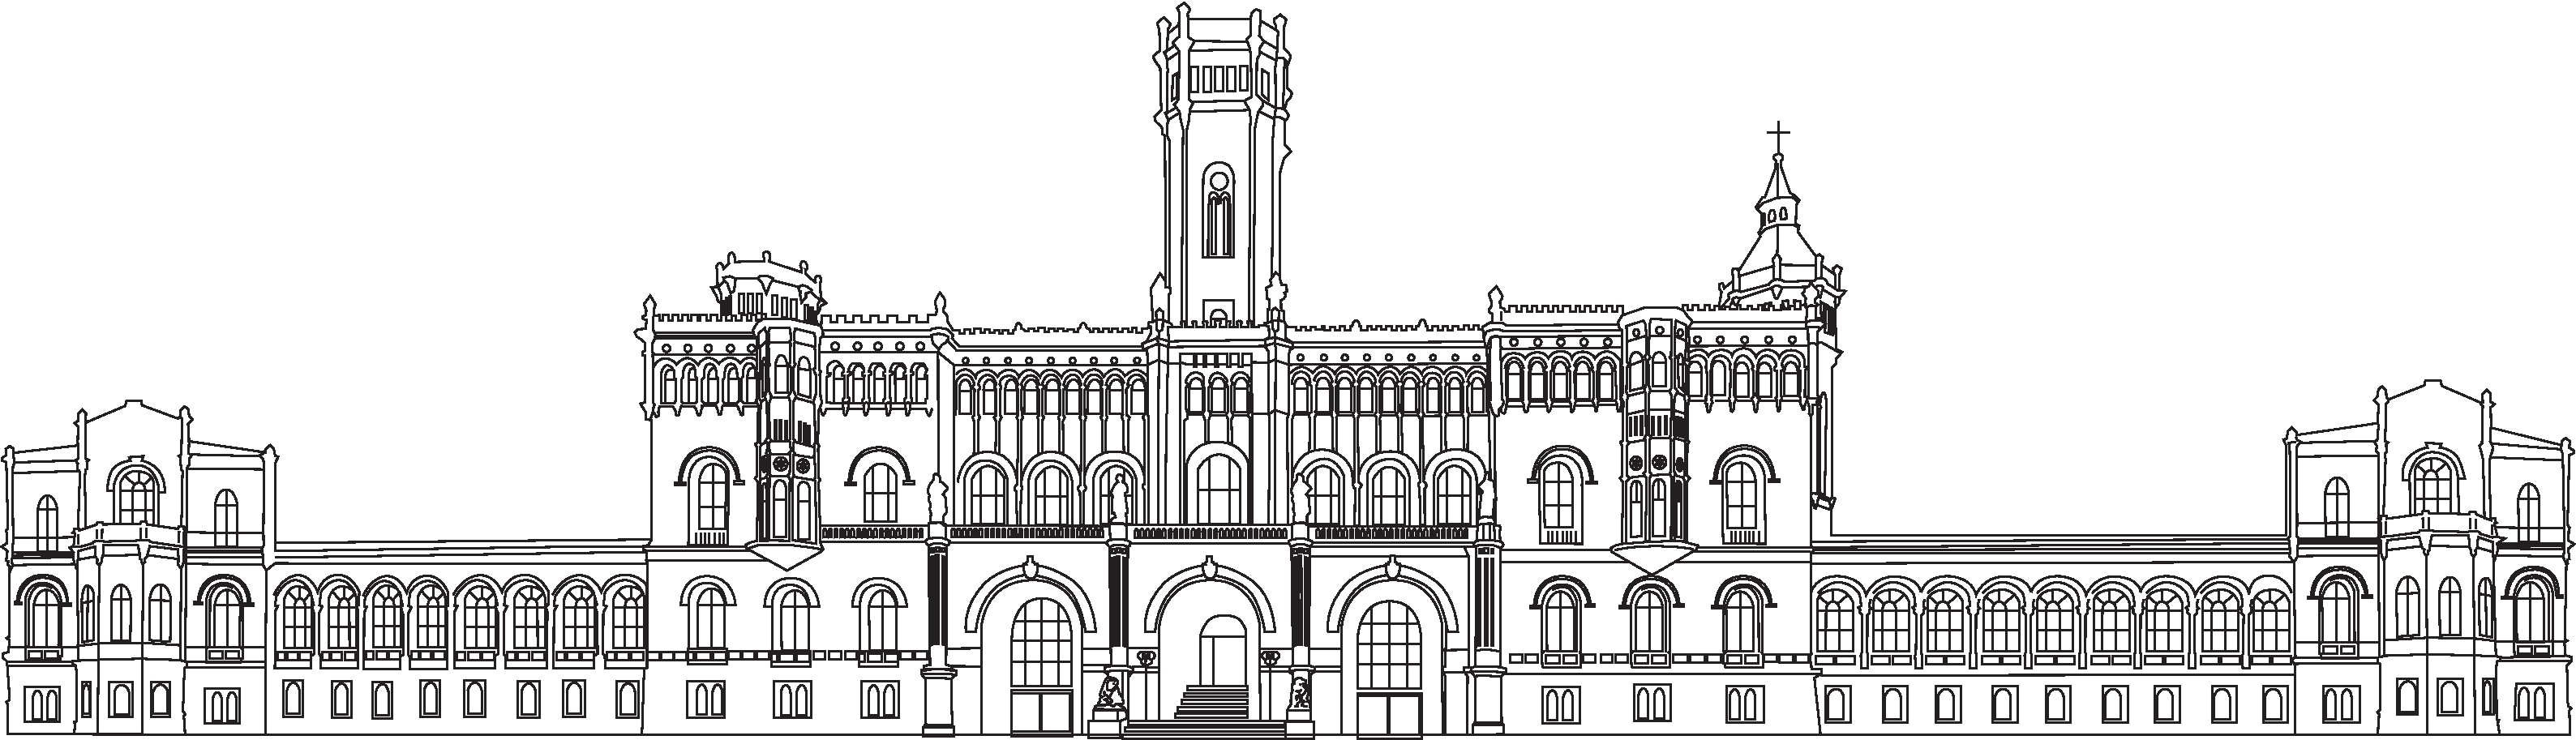
\includegraphics[width=13.8cm]{gfx/welfenschloss} \\ 
  \end{center}
  \medskip
  \begin{center}
    \textbf{\huge\spacedallcaps{L}\LARGE\spacedallcaps{eibniz}}
    \textbf{\huge\spacedallcaps{U}\LARGE\spacedallcaps{niversit\"{a}t}}
    \textbf{\huge\spacedallcaps{H}\LARGE\spacedallcaps{annover}} \\
  \end{center}

  \begin{center}
    \normalsize
    \spacedallcaps{Fakult\"{a}t}
    \spacedallcaps{f\"{u}r}
    \spacedallcaps{Elektrotechnik}
    \spacedallcaps{und}
    \spacedallcaps{Informatik} \\
    \smallskip
    \spacedallcaps{Institut}
    \spacedallcaps{f\"{u}r}
    \spacedallcaps{Kommunikationstechnik}
  \end{center}
  \vfill
  \vfill

  % Start condWIWI
  \condWIWI{
  %*******************************************************
  % Titlepage for Wirtschaftingenieur
  %*******************************************************
  \begin{center}
    \Large \myTitle
  \end{center}
  \vfill
  \vfill

  \begin{center}
    \LARGE \textbf{\myDegree}
  \end{center}
  \vfill

  \begin{center}
    \large zur Erlangung des Grades eines Diplom-Wirtschaftsingenieurs der \\
    \large Fakult\"{a}t f\"{u}r Elektrotechnik und Informatik, Fakult\"{a}t f\"{u}r Maschinenbau und \\
    \large Wirtschaftswissenschaftlichen Fakult\"{a}t der Leibniz Universit\"{a}t Hannover
  \end{center}
  \vfill

  \begin{center}
    \large vorgelegt von \\
  \end{center}
  \medskip

  \begin{center}
    \large \spacedallcaps{\myName}
  \end{center}
  \medskip

  \begin{center}
    \large geb. am \myBirthdate in \myBirthplace \\
  \end{center}

  \vfill
  \vfill

  Pr\"{u}fer: \myProf
  \bigskip

  Hannover, den \myTime
  } 
  {
  %*******************************************************
  % Titlepage for everyone else 
  %*******************************************************
  \begin{center}
    \LARGE \myTitle
  \end{center} 
  \vfill
  \vfill

  \begin{center}
    \LARGE \textbf{\myDegree}
  \end{center}
  \vfill

  \begin{center}
    \large eingereicht von \\
  \end{center}

  \begin{center}
    \large \spacedallcaps{\myName}
  \end{center}

  \begin{center}
    \large am \myTime \\
  \end{center} 
  \vfill

  \begin{center}
    \begin{tabular}{lll}
      Erstpr\"{u}fer  & : & \myProf \\
      Zweitpr\"{u}fer & : & \myOtherProf \\
      Betreuer        & : & \mySupervisor
    \end{tabular}
  \end{center} 

  }  % end condWIWI

%  \vfill

%  \begin{center}
%    \large \selectedthesisnumber \\
%  \end{center}

  \changetext{}{-19mm}{}{-19mm}{}

\end{titlepage}

\thispagestyle{empty}

\hfill

\vfill

\noindent\myName: \textit{\myTitle,} \myDegree, \textcopyright\ \myTime

%\bigskip
%
%\noindent\spacedlowsmallcaps{Supervisors}: \\
%\myProf \\
%\myOtherProf \\ 
%\mySupervisor
%
%\medskip
%
%\noindent\spacedlowsmallcaps{Location}: \\
%\myLocation
%
%\medskip
%
%\noindent\spacedlowsmallcaps{Time Frame}: \\
%\myTime

\cleardoublepage%*******************************************************
% Declaration
%*******************************************************
\refstepcounter{dummy}
\pdfbookmark[1]{Ehrenw\"{o}rtliche Erkl\"{a}rung}{ehrenw\"{o}rtliche erkl\"{a}rung}
\chapter*{Ehrenw\"{o}rtliche Erkl\"{a}rung}
\thispagestyle{empty}

% Start condWIWI
\condWIWI{
%*******************************************************
% Declaration for Wirtschaftingenieur
%*******************************************************
Hiermit versichere ich, dass ich die vorliegende Arbeit selbstst\"{a}ndig verfasst und keine anderen als die angegebenen Quellen und Hilfsmittel benutzt habe, dass alle Stellen der Arbeit, die w\"{o}rtlich oder sinngem\"{a}\ss aus anderen Quellen \"{u}bernommen wurden, als solche kenntlich gemacht sind und dass die Arbeit in gleicher oder \"{a}hnlicher Form noch keiner Pr\"{u}fungsbeh\"{o}rde vorgelegt wurde.
}
{
%*******************************************************
% Delcaration for everyone else 
%*******************************************************
Hiermit versichere ich, die vorliegende \myDegree ohne Hilfe Dritter und nur mit den angegebenen Quellen und Hilfsmitteln angefertigt zu haben. Alle Stellen, die w\"{o}rtlich oder inhaltlich aus den Quellen entnommen wurden, sind als solche kenntlich gemacht worden. Diese Arbeit hat in gleicher oder \"{a}hnlicher Form noch keiner Pr\"{u}fungsbeh\"{o}rde vorgelegen.
} % end condWIWI

\bigskip
 
\noindent\textit{\myLocation, den \myTime}

\smallskip

\begin{flushright}
    \begin{tabular}{m{5cm}}
        \\ \hline
        \centering\myName \\
    \end{tabular}
\end{flushright}

\cleardoublepage%*******************************************************
% Abstract
%*******************************************************
%\renewcommand{\abstractname}{Abstract}
\pdfbookmark[1]{Abstract}{Abstract}
\begingroup
\let\clearpage\relax
\let\cleardoublepage\relax
\let\cleardoublepage\relax

\chapter*{Abstract}
In this thesis I will give an introduction to recommender systems, provide an overview over other recommender system libraries and datasets available to try out the algorithms. After that I will describe different recommender algorithms and evaluation metrics I implemented in my work followed by an explanation on how to use them. Additionally I will provide the result of the tests.


\vfill

\pdfbookmark[1]{Zusammenfassung}{Zusammenfassung}
\chapter*{Zusammenfassung}
Kurze Zusammenfassung des Inhaltes in deutscher Sprache\dots


\endgroup			

\vfill

\cleardoublepage
\pagestyle{scrheadings}
\cleardoublepage%*******************************************************
% Table of Contents
%*******************************************************
%\phantomsection
\refstepcounter{dummy}
\pdfbookmark[1]{\contentsname}{tableofcontents}
\setcounter{tocdepth}{2} % <-- 2 includes up to subsections in the ToC
\setcounter{secnumdepth}{3} % <-- 3 numbers up to subsubsections
\manualmark
\markboth{\spacedlowsmallcaps{\contentsname}}{\spacedlowsmallcaps{\contentsname}}
\tableofcontents 

\cleardoublepage

%\cleardoublepage%*******************************************************
% List of Figures
%*******************************************************    
\automark[section]{chapter}
\renewcommand{\chaptermark}[1]{\markboth{\spacedlowsmallcaps{#1}}{\spacedlowsmallcaps{#1}}}
\renewcommand{\sectionmark}[1]{\markright{\thesection\enspace\spacedlowsmallcaps{#1}}}
%\phantomsection 
\refstepcounter{dummy}
%\addcontentsline{toc}{chapter}{\listfigurename}
\pdfbookmark[1]{\listfigurename}{lof}
\listoffigures

\vspace*{8ex}

\cleardoublepage

%\cleardoublepage%*******************************************************
% List of Tables
%*******************************************************
\automark[section]{chapter}
\renewcommand{\chaptermark}[1]{\markboth{\spacedlowsmallcaps{#1}}{\spacedlowsmallcaps{#1}}}
\renewcommand{\sectionmark}[1]{\markright{\thesection\enspace\spacedlowsmallcaps{#1}}}
%\phantomsection 
\refstepcounter{dummy}
%\addcontentsline{toc}{chapter}{\listtablename}
\pdfbookmark[1]{\listtablename}{lot}
\listoftables

\vspace*{8ex}

\cleardoublepage
%\cleardoublepage%*******************************************************
% List of Listings
%*******************************************************      
\automark[section]{chapter}
\renewcommand{\chaptermark}[1]{\markboth{\spacedlowsmallcaps{#1}}{\spacedlowsmallcaps{#1}}}
\renewcommand{\sectionmark}[1]{\markright{\thesection\enspace\spacedlowsmallcaps{#1}}}
%\phantomsection 
\refstepcounter{dummy}
%\addcontentsline{toc}{chapter}{\lstlistlistingname}
\pdfbookmark[1]{\lstlistlistingname}{lol}
\lstlistoflistings

\vspace*{8ex}

\cleardoublepage

%\cleardoublepage%*******************************************************
% Acronyms
%*******************************************************
\automark[section]{chapter}
\renewcommand{\chaptermark}[1]{\markboth{\spacedlowsmallcaps{#1}}{\spacedlowsmallcaps{#1}}}
\renewcommand{\sectionmark}[1]{\markright{\thesection\enspace\spacedlowsmallcaps{#1}}}
%\phantomsection 
\refstepcounter{dummy}
\pdfbookmark[1]{Abk\"{u}rzungsverzeichnis}{abk\"{u}rzungsverzeichnis}
\markboth{\spacedlowsmallcaps{Abk\"{u}rzungsverzeichnis}}{\spacedlowsmallcaps{Abk\"{u}rzungsverzeichnis}}
\chapter*{Abk\"{u}rzungsverzeichnis}

% Insert your acronyms here
\begin{acronym}[UML]
  \acro{DRY}{Don't Repeat Yourself}
  \acro{API}{Application Programming Interface}
  \acro{UML}{Unified Modeling Language}
\end{acronym}

\cleardoublepage

% ********************************************************************
% Mainmatter
% ********************************************************************
\pagenumbering{arabic}
% use \cleardoublepage here to avoid problems with pdfbookmark
% insert your chapters here
%\cleardoublepage\part{Beispiel einer Arbeit}
\chapter{Introduction}


\section{Motivation}

The library together with this document shall provide a ``cookbook''
for recommender systems. With the simple syntax and the interactivity
of Python it is aimed at beginners to simply experiment with different
algorithms. Especially the interactivity is missing in the already
existing libraries because none of them is written in Python.


\section{Task (what a Recommender System does)}

A Recommender System works in a scenario with users, items and interactions
users can have with items. Such a scenario could be an online shop,
where the interactions are purchases of items by users or a video
platform, where the users interact with items (videos) by watching
them. Based on the past interactions of the users a Recommender System
searches for items a user haven't interacted with yet but the probability
that he will interact is maximized.

The interactions can be implicit like purchases or clicks, then the
scenario is also called item prediction. When the feedback is provided
explicit like ratings the scenario is called rating prediction. In
this work the focus lies on implicit feedback or item prediction.
However ratings can be interpreted as the strength of implicit feedback.
For example how often a user purchased an item. Some algorithms implemented
in this library can use this information but none will explicitly
predict ratings like it's usual in rating prediction scenarios.


\section{Contributions}

The main contribution of my work is the interactive library I wrote
\cite{recsyslab}. Also in this document I provide explanations about
the algorithms implemented in the library and an extensive user manual
of the library.



\chapter{Background}
In this chapter we will provide a short overview over the techniques
used to evaluate recommender algorithms.


\section{Evaluation Methods}

To evaluate a recommender algorithm we have to split up the database
into one for training and one for evaluation. There are different
methods to split the database but in the library only one is implemented
which is the Leave-one-out protocol~\cite{leaveoneout}.
You can use the Leave-one-out protocol with many different metrics
which are also explained here.


\subsection{Leave-one-out Protocol}
\label{leaveoneout}

The Leave-one-out protocol means, that we take one interaction of
each user out of the database for training and use it for validation.
The item the recommender has to predict is also called hidden item. 
Now we can test for each user if the algorithm is capable to predict
this missing interaction. Most of the test metrics described below are counting
how many of the hidden items the algorithm recommends while being
restricted to only recommend a certain number of items. But all
of them take recommendations for each user. This wouldn't be possible
if we would for example just take out 1\% of the interactions it's
likely that there are some users without a hidden item. Then the metrics
wouldn't work anymore.



\subsection{Evaluation metrics}
\label{evaluationmetrics}

These are a selection of different metrics to rate the recommendations.
By default the evaluations are executed with only one hidden item
but generally the metrics should also work with more than just one.

For the notation: U is the set of users, H is the set of hidden items
and \(H_u\) is the set of hidden items for user u. T is the set used for 
training. \(\text{TopN}_u\)
is the set of top N recommendations for user u so the number of items
the recommender is allowed to recommend is N. For the metrics where
the order in which the items are recommended count \(\text{TopN}_u\)
is a list sorted by score in decreasing order.
To get an implicit score of each item the recommender recommends all
items.


\subsubsection{Hitrate/Recall@N}

This metrics lets the recommender recommend N items. If the hidden
item is under the N recommended items, the recommender got a 
hit~\cite{Karypis:2001:EIT:502585.502627, Sarwar00applicationof}.
So the Recall@N is the fraction of users who get recommended a
relevant item when the recommender can recommend N items.
So the hitrate is 

\begin{equation} 
\text{Recall@N}=\frac{\sum_{u \in U} H_u \cap \text{topN}_u}{|H|}
\end{equation}


This metric is very intuitive you can for example imagine that you
show the user 10 items then Recall@10 would be the chance of showing
the user an item he will interact with. But this metric doesn't take
the number of recommended items into account.


\subsubsection{Precision}

The precision~\cite{Sarwar00applicationof} is 

\begin{equation} 
\text{Precision}=\frac{\sum_{u \in U} H_u \cap \text{topN}_u}{N \times |U|}
\end{equation}


As you can clearly see this metric is taken the number of recommended
items into account. Which will probably lead to worse results as the
number of recommended items increases.


\subsubsection{F1}

The F1 metric~\cite{Sarwar00applicationof} tries to balance hitrate and precision
by taking both into account.

\begin{equation}
\text{F1}=\frac{2 \times \text{Recall@N} \times \text{Precision}}{\text{Recall@N} + \text{Precision}}
\end{equation}


\subsubsection{Mean Reciprocal Hitrate}

The mean reciprocal hitrate or more general mean reciprocal
rank~\cite{DBLP:conf/icdm/NingK11} counts the hits but punishes them the more the lower they
appear in the list of recommendations. So if the hidden item appears
first in the list of recommendations the hit counts as one, but when
it is in the second position the hit already counts only as one half
and so on.

\begin{equation}
\text{MRHR}=\frac{1}{|U|} \sum_{u \in U} \frac{1}{\text{pos}(\text{topN}_{u},H_{u})}
\end{equation}

Where N is the number of items in the dataset and \(\text{pos}(\text{topN}_{u},H_{u})\)
is the position of the hidden item in the recommendation.


\subsubsection{Area under the ROC (AUC)}

AUC~\cite{Rendle:2009:BBP:1795114.1795167} counts the number of items the recommender rates
higher than the hidden item, normalize it by the number of items the
recommender can rate higher. Sum this up for every user and again
normalize by the number of users.

To get an implicit score of each item the recommender recommends all
items in a list sorted by score in decreasing order. This is in fact the same
as for the other metrics only that the recommender can recommend as
many items as possible.

\begin{equation}
\text{AUC}=\frac{1}{|U|}\sum_{u \in U} \frac{1}{|E(u)|} \sum_{(i,j) \in E(u)} \delta(x_{ui}>x_{uj})
\end{equation}

Where \(x_{ui}\) is the predicted score of the interaction between User u and item i.
\(\delta\) is defined as follows
\begin{equation}
\delta(x)=\begin{cases}1, & \text{if x is true} \\
                       0, & \text{otherwise}
\end{cases}
\end{equation}

And \(E(u)\) is 
\begin{equation}
E(u) =\{(i,j)|(u,i) \in H \land (u,j) \not\in (H \cup T)\}
\end{equation}


\section{Datasets for testing}

In the WWW there are several anonymized datasets available to try
out recommender systems and to evaluate their performance. 
Following we will introduce three of them.


\subsection{MovieLens}
\label{movielens}

MovieLens~\cite{movielensdatasets} is a database provided by GroupLens, a research
lab at the University of Minnesota. One of their research areas is
recommender systems and they built an application where users rate
movies and then get recommendations for movies the could like. The
MovieLens dataset is the ratings gathered by this application. For
this work we will interpret the rating as intensity of interaction
between users and items for example the number of times the user saw
this movie.

The dataset is available in three different sizes:
\begin{itemize}
\item 100,000 interactions
\item 1 million interactions
\item 10 million interactions
\end{itemize}
For the experiments the smallest dataset is totally sufficient, with
the larger datasets the computation time gets too long for just trying
something out.


\subsection{Million Song Dataset}
The million song dataset~\cite{Bertin-Mahieux2011} is a large database of features and media data
of a million songs. For a challenge they also provided the listening history of over 1 million
user. To present I will use a subset of this dataset to keep the computing time required
reasonable low so it's easier for others to retrace the results.


\subsection{476 Million Twitter Tweets Dataset}
The Stanford Network Analysis Project provided a twitter dataset with about 467 million tweets from 17.000 users~\cite{snap}.
Unfortunately the dataset is no more available. [further explanation or deletion]
To convert the tweets two user item interactions I will interpret the hashtags[explanation necessary?] as items.
So tweets of a user with a hashtag is a interaction between the user and the hashtag.


\chapter{Related Work}
\label{relatedwork}

There is a wide range of projects providing implementations for recommender
system. Some of them are described in this chapter to give a quick
overview and comparison.


\section{MyMediaLite}

MyMediaLite~\cite{Gantner2011MyMediaLite} is an open source project developed at the
University of Hildesheim and provides several algorithms for rating
prediction and item prediction. It is written in C\# and can be used with
a command line interface. It also provides a graphical interface to
demonstrate recommender algorithms.


\section{PREA (Personalized Recommendation Algorithms Toolkit)}

PREA~\cite{2012arXiv1205.3193L} is an open source project written in Java. It provides
a wide range of recommender algorithms and evaluation metrics to test
them. It is maintained by the Georgia Institute of Technology.


\section{Apache Mahout}

Mahout~\cite{mahout} is an open source library in Java. It is implemented
on top of Apache Hadoop, so it uses the map/reduce paradigm. This
means it can run on different, independent computers.


\section{Duine Framework}

The Duine Framework~\cite{duine} is an open source project written
in Java by the Telematica Instituut/Novay. The recommender of the
Duine Framework combines multiple prediction techniques to exploit
the strengths of the different techniques and to avoid their weaknesses.


\section{Cofi}

Cofi~\cite{cofi} provides an algorithm for the rating prediction
task called Maximum Margin Matrix Factorization. It is open source
and written in C++.


\section{LensKit}

Lenskit~\cite{Ekstrand:2011:RRR:2043932.2043958} is a toolkit which provides several recommender
algorithms and an infrastructure to evaluate them. It is an open source
project by the University of Minnesota.


\section{Comparison}
The table below compares the algorithms implemented by the different
frameworks.

\begin{table}[h]
\scalebox{0.53}{
\begin{tabular}{c|l|cccccc} \toprule
    Category & Feature & PREA & Mahout & Duine & Cofi & MyMedia & \textbf{recsyslab}\\ \midrule
    \multirow{2}{*}{Baselines} & Constant & O & & & O & O & O\\
                               & User/Item Average & O & O & O &O&O& \\
                               & Random &O&&&&O&O\\\midrule
    \multirow{3}{*}{Memory-based CF}& User-based CF~\cite{su2009survey}&O&O&O&O&O&O\\
                                    & Item-based CF~\cite{linden2003amazon}&O&O&O&O&O&O\\
                                    & Default Vote, Inf-User-Frex~\cite{breese1998empirical}&O&O&&&&\\
                                    & Slope-One~\cite{lemire2005slope}&O&O&&&O&O\\ \midrule
    \multirow{6}{*}{Matrix Factorization}&SVD~\cite{paterek2007improving}&O&O&&O&O&O\\
                                         &NMF~\cite{seung2001algorithms}&O&&&&&\\
                                         &PMF~\cite{salakhutdinov2008probabilistic}&O&&&&&\\
                                         &Bayesian PMF~\cite{salakhutdinov2008bayesian}&O&&&&&O\\
                                         &Non-linear PMF~\cite{lawrence2009non}&O&&&&&\\
                                         &RankMFX~\cite{diaz2012happening}&&&&&&O\\ \midrule
    \multirow{2}{*}{Other methods}       &Fast NPCA~\cite{yu2009fast}&O&&&&&\\
                                         &Rank-based CF~\cite{sun2012estimating}&O&&&&&\\ \midrule
    \multirow{5}{*}{Evaluation Metric}   &(N)MAE&O&O&O&O&O&\\
                                         &RMSE&O&O&&O&O&\\
                                         &HLU/NDCG&O&&&&O&\\
                                         &Kendall's Tau, Spearman&O&&&&&\\
                                         &Precision/Recall/F1&&O&&&O&O\\
                                         &ARHR/MRHR&&&&&&O\\ \midrule
    \multirow{6}{*}{Miscelaneous}        &Sparse Vector/Matrix&O&O&O&O&O&O\\
                                         %&Wrapper for other languages&O&&&O&O&\\
                                         &Item Recommender for Positive-only Data&&&&&O&O\\
                                         &Release Year&2011&2005&2009&2004&2009&2013\\
                                         &Language&Java&Java&Java&C++&C\#&Python\\
                                         &License&GPL&LGPL&LGPL&GPL&GPL&GPLv3\\ \bottomrule
\end{tabular}}
\label{comparisontable}
\caption{Comparison of different recommender frameworks}
\end{table}

\chapter{Recommendation Algorithms}
\label{recommendationalgorithms}
In this chapter we will provide an overview on how the algorithms we implemented
work. To illustrate the simplicity of the code we will also show the core part of 
the source code of the respective recommender algorithm.
For further explanations please refer to the cited papers.


\section{Non-Personalized Algorithms}

In this section we will describe two very simple and basic recommendation
algorithms we implemented for comparison with the more sophisticated
algorithms.


\subsection{Constant}

The constant recommender algorithm counts the number of interactions
for each item and sorts this in decreasing order of interactions.
Then it recommends the top items of this list. So it recommends the
items which are the most popular over all users and does not do any
personalizations. The intuition here is that the most popular items
will be interesting for everyone. However the results show that
algorithms which personalize the recommendation based on the 
interaction history of the users perform much better.
In pseudocode this algorithm will look like this:
\begin{lstlisting}[style=pseudocode]
countDict = dict initialized with all ItemIDs as keys and 0 as values

for interaction in dataset:
    countDict(ItemID(interaction))++

ranking = list(ItemIDs in decreasing order of their values)

return first N items of ranking
\end{lstlisting}
And the implementation:
\begin{lstlisting}[style=python]
def __init__(self, dbdict):
    self.dictionary = {}
    self.sortedList = []
    for data in dbdict.iteritems():
        for item, rating in iter(data[1]):
            if item in self.dictionary:
                self.dictionary[item] += rating
            else:
                self.dictionary[item] = rating

    self.sortedList = helper.sortList(self.dictionary.iteritems())

def getRec(self, user, n):
    return self.sortedList[:n]
\end{lstlisting}



\subsection{Random}

The random recommender algorithm chooses items to recommend randomly.
Even though this algorithm will recommend different items for different
users it is not personalized because it the recommendations are
independent of the previous interactions of the user.
In pseudocode this will be:
\begin{lstlisting}[style=pseudocode]
return N randomly chosen items
\end{lstlisting}
And in Python:
\begin{lstlisting}[style=python]
def __init__(self, dbdict, seed):
    self.maxIid = 0
    self.seed = seed
    for data in dbdict.iteritems():
        for itemRating in iter(data[1]):
            item = itemRating[0]
            if item > self.maxIid:
                self.maxIid = item
    self.maxIid += 1

def getRec(self, user, n):
    random.seed(self.seed)
    if self.maxIid < n or n == -1:
        l = range(self.maxIid)
        random.shuffle(l)
        return l
    return list(random.sample(range(self.maxIid), n))
\end{lstlisting}


\section{k-Nearest-Neighbor}

This class of recommendation algorithms works by searching neighbors
of either items or users based on a similarity function which is the
cosine in this library. The similarity function is interchangeable 
for example in
\cite{Karypis:2001:EIT:502585.502627} two similarity functions are
compared. The cosine similarity performs best so in recsyslab only the cosine similarity
is implemented. For two vectors \(\vec{v},\vec{u}\)
The cosine similarity is defined as follows:

\begin{equation}
\cos(\vec{v}, \vec{u})=\frac{\vec{v} \cdot \vec{u}}{||\vec{v}||_{2} ||\vec{u}||_{2}}
\end{equation}
With the similarity it is possible to rank items.
In the Item Based algorithm for each item we compute the sum of 
similarities with the items the user already bought and rank 
accordingly.
In the User Based algorithm for every item we sum up the 
similarities of the user who bought this item and rank
according to this score.


\subsection{Item Based}
\label{itembasedknn}

For this algorithm the database has to be represented as a matrix
where the rows correspond to the users and the columns to the items.
Then the entry (i,j) represents the number of transactions which happened
between the i-th user and the j-th item. 

The algorithm interprets the columns of the matrix i.e. the items
as vectors and computes there similarities by computing their cosine.
To build the model the algorithm computes the n most similar items
of each item. In pseudocode:
\begin{lstlisting}[style=pseudocode]
for every item i
    for every item j
        sim[i,j] = similarity between i and j

for every item i
    for every item j
        if sim[i,j] not one of the n largest in sim[i]
            sim[i,j] = 0
\end{lstlisting}
In Python it looks like this:
\begin{lstlisting}[style=python]
def __init__(self, userItemMatrix, n):
    self.itemUserMatrix = userItemMatrix.transpose()
    self.sim = computeCosSim(self.sim, self.itemUserMatrix)
    self.userItemMatrix = userItemMatrix

    order = self.sim.argsort(1)

    # for each row in sim:
    # Set all entries to 0 except the n highest
    for j in xrange(0, self.sim.shape[1]):
        for i in xrange(0, self.sim.shape[1] - n):
            self.sim[j, order[j, i]] = 0
\end{lstlisting}
\lstinline!computeCosSim! looks like this:
\begin{lstlisting}[style=python]
def computeCosSim(sim, matrix):
    for i in xrange(1, sim.shape[1]):

        for j in xrange(0, i):
            sim[i, j] = sim[j, i] = cos(
                matrix[i], matrix[j])
    return sim
\end{lstlisting}
This function is also used in the user based k-Nearest-Neighbor.


To compute recommendations for user $U$ the algorithm computes
the union of the n most similar items of each item $U$ interacted with.
From this set the items $U$ already interacted with are removed. For
each item remaining in this set we compute the sum of its similarities
to the items $U$ interacted with. Finally these items are sorted in
decreasing order of this sum of similarities and the first n items
will be recommended~\cite{Karypis:2001:EIT:502585.502627}.
The pseudocode is
\begin{lstlisting}[style=pseudocode]
for every item i user u bought
    itemSimVector = itemSimVector + vector of i

for every item i user u bought
    itemSimVector[i] = 0

return the N items with the highest value in itemSimVector
\end{lstlisting}
The Python equivalent:
\begin{lstlisting}[style=python]
def getRec(self, u, n):
    # x are the similarities of each item to the items u bought
    # w.r.t. only the highest n similarities are saved.
    x = self.userItemMatrix[u] * self.sim

    # Throw out items the user already purchased
    for i in xrange(0, self.sim.shape[0]):
        if self.userItemMatrix[u, i] != 0:
            x[0, i] = 0

    order = x.argsort()
    l = []
    for i in xrange(1, n + 1):
        l.append(order[0, -i])
    return l
\end{lstlisting}



\subsection{User Based}

The user based k-Nearest-Neighbor~\cite{userbasedknn} is very similar to the item based.
But instead of interpreting the columns as vectors, we interpret the
lines or users of the matrix as vectors and compute their similarities
to other users.
Pseudocode:
\begin{lstlisting}[style=pseudocode]
for every user u
    for every user o
        sim[u,o] = similarity between u and o

for every user u
    for every user o
        if sim[u,o] not one of the n largest in sim[u]]
            sim[u,o] = 0
\end{lstlisting}
Python:
\begin{lstlisting}[style=python]
def __init__(self, userItemMatrix, n):
    self.userItemMatrix = userItemMatrix
    self.sim = np.zeros((userItemMatrix.shape[0], userItemMatrix.shape[0]))
    self.sim = computeCosSim(self.sim, self.userItemMatrix)

    order = self.sim.argsort(1)

    # for each row in sim:
    # Set all entries to 0 except the n highest
    for j in xrange(0, self.sim.shape[1]):
        for i in xrange(0, self.sim.shape[1] - n):
            self.sim[j, order[j, i]] = 0
\end{lstlisting}


Then for each item i we sum up the similarities between $U$ and the
users who interacted with i. Again we remove all items $U$ already interacted
with, sort in decreasing order fo the sum and recommend the first
n items.
Pseudocode:
\begin{lstlisting}[style=pseudocode]
for every item i 
    for every user o
        score(i) = score(i) + sim[U,o]

for every item i user u bought
    score(i) = 0

return the N items with the highest value in score
\end{lstlisting}
Python:
\begin{lstlisting}[style=python]
def getRec(self, u, n):
    # x is the weighted sum of the items
    # weighted with the similarity between u and the
    # other users.
    x = self.sim[u] * self.userItemMatrix

    for i in xrange(0, self.sim.shape[0]):
        if self.userItemMatrix[u, i] != 0:
            x[0, i] = 0

    order = x.argsort()
    l = []
    for i in xrange(1, n + 1):
        l.append(order[0, -i])

    return l
\end{lstlisting}

\section{Matrix Factorization}
As mentioned in Section~\ref{matrixfactorization} the matrix factorization
techniques generate two matrices \(W\) and \(H\) so that \(\hat{M} = W\;H^\top\).
Each of the implemented algorithms train these two matrices with stochastic
gradient descent. In each iteration the model is trained with
\begin{itemize} 
    \item a randomly chosen user $U$
    \item a randomly chosen item $I$ the user $U$ interacted with, called the positive item and 
    \item a randomly chosen item $J$ the user $U$ did not already interacted with, 
        called the negative item.
\end{itemize}
The features of $U$, $I$ and $J$ are trained using the derivative
of a loss function.

BPRMF and RankMFX are sharing the code in the module \lstinline!recommender.mf!. 
The only difference is the loss function.
In pseudocode the model update happening in each iteration looks like this:
\begin{lstlisting}[style=pseudocode]
U = randomly chosen user
I = randomly chosen item U interacted with
J = randomly chosen item U did not interact with

X=H[i] - H[j]
wx = dot product of W[u] and X
dloss = (derivative of the loss function of wx and 1) * learningRate

W[u] += dloss * (H[i] - H[j]) # These three lines
H[i] += dloss * W[u]          # have to be
H[j] += dloss * -W[u]         # executed at once
\end{lstlisting}
The Python code doing the same looks like this:
\begin{lstlisting}[style=python]
u = random.choice(R.keys())

userItems = [x[0] for x in R[u]]
# the positive example
i = userItems[np.random.random_integers(0, len(userItems) - 1)]
# the negative example
j = np.random.random_integers(0, m_items)
# if  j is also relevant for u we continue
# we need to see a negative example to contrast the positive one
while j in userItems:
    j = np.random.random_integers(0, m_items)

X = H[i] - H[j]
wx = np.dot(W[u], X)
dloss = dlossF(wx, y)

# temp
wu = W[u]
hi = H[i]
hj = H[j]

if dloss != 0.0:
    # Updates
    eta_dloss = learningRate * dloss
    W[u] += eta_dloss * (hi - hj)
    H[i] += eta_dloss * wu
    H[j] += eta_dloss * (-wu)

    W[u] *= scaling_factorU
    H[i] *= scaling_factorI
    H[j] *= scaling_factorJ
\end{lstlisting}
For the recommendations we rank the items with a score.
The score of an item for a user is the dot
product of the feature vector of the user 
and the feature vector of the item. All matrix factorization
algorithms use this.
In pseudocode:
\begin{lstlisting}[style=pseudocode]
for every item i
    scoreList(i) = W[u] * H[i]

sortByScore(score)
return first N of score
\end{lstlisting}
And in Python:
\begin{lstlisting}[style=python]
def getRec(self, u, n):
    scoredict = {}
    for i in range(0, self.H.shape[0]):
        if not i in [x[0] for x in self.R[u]]:
            scoredict[i] = np.dot(self.W[u], self.H[i])

    if n == -1:
        n = len(scoredict)
    import util.helper
    return util.helper.sortList(scoredict.iteritems())[:n]
\end{lstlisting}


\subsection{BPRMF}

In our implementation of BPMRF we use the logLoss to train the model. The logLoss is defined
as
\begin{equation}
\textrm{logLoss}(a,y)=\log(1+\exp(-ay)).
\end{equation}
And the derivative of the logLoss is
\begin{equation}
\frac{\partial}{\partial y}(\textrm{logLoss})=-\frac{a}{\exp(ay)+1}.
\end{equation}
For further informations please refer to~\cite{Rendle:2009:BBP:1795114.1795167}


\subsection{RankMFX}

RankMFX uses the hingeLoss. It is defined as

\begin{equation}
\mathrm{\textrm{hingeLoss}(a,y)=\max(0,1-ay)}.
\end{equation}
And its derivative

\begin{equation}
\frac{\partial}{\partial y}(\textrm{hingeLoss})=\begin{cases}
-y, & ay<1,\\
0, & \textrm{otherwise}.
\end{cases}
\end{equation}
See also~\cite{diaz2012happening}.


\subsection{Ranking SVD (Sparse SVD)}

Ranking SVD uses the quadratic loss and the difference between the
predicted score of the positive item and the negative minus the actual
score of the positive item~\cite{jahrer2011collaborative}.
Ranking SVD uses code different from BPRMF and RankMFX, but the iterations
work the same. It also randomly chooses a user and a positive and a
negative item in each iteration of the stochastic gradient descent. 
But the model updates are different. In pseudocode:
\begin{lstlisting}[style=pseudocode]
U = randomly chosen user
I = randomly chosen item U interacted with
J = randomly chosen item U did not interact with

ruipred = W[U] * H[I] # Prediction for item I
rujpred = W[U] * H[J] # Prediction for item J
rui = actual value of the interaction between U and I 
ruj = 0

dloss = (ruipred - rujpred) - (rui - ruj)
W[U] = W[U] - learningRate * dloss * (H[I] - H[J])
H[I] = H[I] - learningRate * dloss * W[U]
H[J] = H[J] - learningRate * dloss * -W[U]
\end{lstlisting}
And in Python this part looks like this:
\begin{lstlisting}[style=python]
# Choose an user randomly
u = random.choice(R.keys())
# Choose an item the user interacted with
userItems = [x[0] for x in R[u]]
i = random.choice(userItems)
# Choose an item, the user didn't interacted with
i0 = np.random.random_integers(0, m_items - 1)
while i0 in userItems:
    i0 = np.random.random_integers(0, m_items - 1)

# Prediction for the first item
ruipred = userFeatures[u].dot(itemFeatures[i])
# Prediction for the second item
rui0pred = userFeatures[u].dot(itemFeatures[i0])
rui0 = 0
for r in R[u]:
    if r[0] == i:
        rui = r[1]

dloss = (ruipred - rui0pred) - (rui - rui0)
c = userFeatures[u]
userFeatures -= learningRate * dloss * (
    itemFeatures[i] - itemFeatures[i0])
itemFeatures[i] -= learningRate * dloss * c
itemFeatures[i0] -= learningRate * dloss * (-c)
\end{lstlisting}


\section{Other}
In this section we will describe one last algorithm 
which does not fit into the above categories.
\subsection{Slope One}
The Slope One recommendation algorithm computes the differences of
interaction intensities between items and uses these differences to 
predict indirectly the interaction intensity between users and items
without any interaction~\cite{DBLP:journals/corr/abs-cs-0702144}.
The model building in pseudocode:
\begin{lstlisting}[style=pseudocode]
for all interaction pairs i, j where i != j
    diffs[i][j] = i.rating - j.rating
    count[i][j]++
\end{lstlisting}
And in Python:
\begin{lstlisting}[style=python]
def __init__(self, R):
    self.diffs = {}
    self.R = R

    for u in R.keys():
        for i, r in R[u]:
            if not i in self.diffs:
                self.diffs[i] = {}

            for i1, r1 in R[u]:
                if i == i1:
                    continue
                if not i1 in self.diffs[i]:
                    self.diffs[i][i1] = [0.0, 0.0]

                self.diffs[i][i1][0] += r - r1
                self.diffs[i][i1][1] += 1
\end{lstlisting}
For the recommendations for every item, we sum up its differences with
the items the user rated, together with the rating the user gave these
other items. Additionaly this is multiplied by the number of times the
difference occured. This is then normalized by the sum of the occurrences
of the differences. The following pseudocode clarifies this.
\begin{lstlisting}[style=pseudocode]
for every item i
    ratingSum = 0
    count = 0
    for every item j user u interacted with
        ratingSum = ratingSum + ((rating u gave j) 
                              + diffs[i][j])
                              * count[i][j]
        count = count + count[i][j]

    ratingSum /= count
    listToRecommend.add( (i, ratingSum))

sortAfterRatingSum(listToRecommend)
return first N of listToRecommend
\end{lstlisting}
And in python:
\begin{lstlisting}[style=python]
def getRec(self, u, n):
    maxIid = max(self.diffs.keys())
    userItems = [x[0] for x in self.R[u]]
    predictionList = []

    for i in xrange(0, maxIid + 1):
        if i in userItems:
            continue

        ratingSum = 0
        count = 0
        for i1, r in self.R[u]:
            if i in self.diffs:
                if i1 in self.diffs[i]:
                    ratingSum += (r + self.diffs[i][i1][0]
                                    ) * self.diffs[i][i1][1]
                    count += self.diffs[i][i1][1]

        if count == 0:
            continue
        ratingSum /= count
        predictionList.append((i, ratingSum))

    import util.helper
    sortedList = util.helper.sortList(predictionList)

    return sortedList[:n]
\end{lstlisting}

\chapter{Experiments}
\label{experiments}
In this chapter we will show test results of every metric with every
recommender algorithm and how they were computed.


\section{Execution}
The results were computed using the recommender algorithms and 
the test metrics implemented in recsyslab. It was done 
like it is shown in the user manual in~\ref{usermanual}.
with exact the same parameters.
The only difference is that for simplification the different
getRec methods and metric methods were each in a list and the 
algorithm is iterating trough both in two nested for loops
to guarantee that every algorithm is tested with every metric.
The code which generated the table in \ref{results} is in 
the experiments.py file in the bin directory of recsyslab.
So check it out for further implementation details.


\section{Results}
\label{results}
Here are the results of every test metric in recsyslab
with every recommender algorithm in recsyslab.

\vspace{1.5 mm}
\begin{tabular}{rlllll}
    recommender  & hitrate & precision & f1 & mrhr & auc \\ \midrule
    constant & 0.0731 & 0.0073 & 0.1448 & 0.0207 & 0.8263 \\
    randomRec & 0.0053 & 0.0005 & 0.0104 & 0.0011 & 0.4790 \\
    itemKnn & 0.2576 & 0.0257 & 0.5099 & 0.1151 & 0.8687 \\
    userKnn & 0.2619 & 0.0261 & 0.5183 & 0.1203 & 0.9279 \\
    BPRMF& 0.2492 & 0.0249 & 0.4931 & 0.0996 & 0.9294 \\
    RankMFX & 0.1792 & 0.0179 & 0.3546 & 0.0686 & 0.8295 \\
    Ranking SVD & 0.1198 & 0.0119 & 0.2371 & 0.0339 & 0.7725 \\
    slopeone & 0.0858 & 0.0085 & 0.1699 & 0.0350 & 0.4699 \\ \bottomrule
\end{tabular}

\newpage
\section{Comparison}
To show the performance of recsyslab we compare our test results with results 
from this paper:~\cite{deshpande2004item}

\vspace{1.5 mm}
\begin{tabular}{rllll} \toprule
 & \multicolumn{2}{c}{hitrate} & \multicolumn{2}{c}{mrhr} \\ \cmidrule(r){2-3} \cmidrule(r){4-5}
 & recsyslab & \cite{deshpande2004item} & recsyslab & \cite{deshpande2004item} \\ \midrule
    constant & 0.0731 & 0.131 & 0.0207 & 0.046 \\
    itemKnn & 0.2576 & 0.271 & 0.1151 & 0.119 \\
    userKnn & 0.2619 & 0.281 & 0.1203 & 0.128 \\ \bottomrule
\end{tabular}
\vspace{1.5 mm}

It can be seen that recsyslab performs almost as good as the reference.
The small advantage probably comes from normalization we did not use when
we were computing these results.


\chapter{Design and Implementation}
In this chapter we'd like to give a quick overview over the library
by explaining the overall structure of the library and how to extend it.


\section{General structure}
One important part is the reader class in the util package.
While the reader reads the dataset it maps the UserIDs and 
ItemIDs from the original IDs in the dataset to internal IDs 
starting at zero and counting up to guarantee that the IDs are consecutive. 
When the IDs are consecutive it's for example possible to use them as
indices in a matrix. \\Furthermore the reader constructs a dict and a matrix
out of the data using the internal IDs. The dict has the internal 
UserIDs as keys and the values are tuples representing the 
interactions of the corresponding user. The first value of these tuples is the internal
ItemID of the interaction, the second is the intensity or
quantity of the interaction. You get the dict by calling \lstinline!getR()!
of the reader object.\\
The matrix offered by a reader has as much lines as the dataset
has users and as much columns as items are present in the dataset.
The entry at the ith line and jth column is then the intensity of the interaction
between user i and item j. A zero means that there hasn't been any
interaction yet.

The k-Nearest-Neighbor algorithms need a matrix like it is provided by a
reader. All other recommendation algorithms need a dict of the 
form described above.

\section{Interfaces}



\chapter{User Manual}
In this chapter I will provide a user manual for the library I implemented\cite{recsyslab}.
First, I will explain how to load a dataset, second I
will explain how to use the different recommendation algorithms and
how to test them with the provided test metrics. For informations about
the recommendation algorithms, please refer to \ref{recommendationalgorithms}.
For informations about the test metrics refer to \ref{evaluationmetrics}.
Also for help you can use the inline documentation available as docstrings.
The following python code is also in the file manual.py in the bin directory of the library
so you don't have to copy the code out of this pdf document.
You can display them with the command line utility
pydoc\footnote{I will use \$ to indicate a bash prompt.}. So for example when you're in the
bin directory of the library call

\begin{lstlisting}
$ pydoc __init__
$ pydoc util 
$ pydoc recommender.BPRMF
\end{lstlisting}

Each of these commands will show the documentation of the specified module.


\section{Load the Dataset}
To load the dataset it has to be a textfile where each line is of the following format:
\begin{lstlisting}
UserID<string>ItemID<string>NumberOfInteractions
\end{lstlisting}
<string> is an arbitrary string but it has to be the same throughout the whole dataset.
NumberOfInteractions is optional and can be omitted and one will be assumed.
Everything coming after NumberOfInteractions<string> will be ignored.
Please note that when you're omitting NumberOfInteractions but have something else after
the ItemId, this will be recognized as NumberOfInteractions.
I recommend to use the MovieLens database\ref{movielens} with 100,000 ratings.
It is easy to get, doesn't need any modifications to work with my library and has a
reasonable size. Also I will use this dataset in the following examples.

When you have a suiting database, start up a python interpreter of version 2.7.x.
\begin{lstlisting}
$ python
\end{lstlisting}

Now import the util.reader module and initialize a new reader object with
\footnote{I will use >>> to indicate the python prompt.}
\begin{lstlisting}
>>> import util.reader
>>> r=util.reader.stringSepReader("u.data","\t")
Start reading the database.
10000 Lines read.
20000 Lines read.
30000 Lines read.
40000 Lines read.
50000 Lines read.
60000 Lines read.
70000 Lines read.
80000 Lines read.
90000 Lines read.
100000 Lines read.
\end{lstlisting}
Note that it outputs the progress it has already made.
The first parameter of the constructor is the name of the file containing the dataset,
the second the string which is separating the values, here it is a tab. 
When you are using another dataset you probably have to change the filename and perhaps
also the separating string.
The constructor creates a mapping from the original IDs to internal IDs both for the users
and the items to make sure that the IDs are consecutive. So to get the items a user interacted
with we have to first find out the internal UserID.
\begin{lstlisting}
internalID=r.getInternalUid("196")
>>> r.getR()[internalID]
set([(521, 1), (377, 4), (365, 3), (438, 5), (86, 4), (649, 4), (0, 3), (522, 3), (423, 3), (389, 5), (751, 3), (656, 4), (947, 4), (432, 2), (632, 2), (431, 5), (221, 5), (92, 4), (291, 3), (528, 4), (83, 4), (363, 3), (466, 4), (289, 5), (512, 5), (179, 3), (329, 4), (672, 4), (834, 5), (665, 3), (321, 2), (487, 3), (380, 4), (1006, 4), (1045, 3), (491, 3), (302, 4), (550, 5), (10, 2)])
\end{lstlisting}
r.getR() returns a dict with internal UserIDs as keys and sets of (ItemID, NumberOfInteractions) tuples.
Please note that the original ID is a string.

To evaluate the algorithms you have to split the datasets like described at \ref{leaveoneout}.
You do this by calling
\begin{lstlisting}
>>> import util.split
>>> trainingDict, evaluationDict = util.split(r, 1234567890)
0 Users split.
100 Users split.
200 Users split.
300 Users split.
400 Users split.
500 Users split.
600 Users split.
700 Users split.
800 Users split.
900 Users split.
\end{lstlisting}
This will split a dict like r.getR() returns into a trainingDict where one transaction
per user is missing and an evaluationDict with these missing transactions.


\section{Non-Personalized Algorithms}
To make our first simple recommendations with the constant recommender
we need to initialize an object of the constant class.
As parameter the constructor needs a dict for training
\begin{lstlisting}
import recommender.nonpersonalized
constant = recommender.nonpersonalized.constant(r.getR())
constant.getRec(0, 10)
\end{lstlisting}
Every recommender has a getRec function with this signature. The first paramater is the internal
UserID, the second is the number of items to be recommended. If n = -1 all items get recommendend.
Also the IDs of the recommended items are internal ones.
If you want to pass external UserIDs and get external ItemIDs back you don't have
to map them all by yourself. Instead you can use a helper function called
getExternalRec.
\begin{lstlisting}
import util.helper
externalConstantgetRec = 
    util.helper.getExternalRec(constant.getRec, r)
externalConstantgetRec("196", 10)
\end{lstlisting}
You pass the getRec function and the reader object and you get a new function
which takes and returns only the original IDs.

Now we want to find out how good this algorithm is performing.
Excpet AUC the functions for computing the metrics work by letting the recommender recommend
for every user as much items as specified in the third parameter.
With these recommendations and the hidden items the methods then calculate the
performance according to the respective metric.
The other parameters are a dict with the hidden items and the getRec function of the 
respective recommender algorithm.

First we will compute the hitrate
\begin{lstlisting}
>>> import util.test
>>> hits, items = util.test.hitrate(evaluationDict, constant.getRec, 10)
0 users tested
Hits so far: 0.0
100 users tested
Hits so far: 4.0
200 users tested
Hits so far: 14.0
300 users tested
Hits so far: 26.0
400 users tested
Hits so far: 31.0
500 users tested
Hits so far: 40.0
600 users tested
Hits so far: 49.0
700 users tested
Hits so far: 52.0
800 users tested
Hits so far: 61.0
900 users tested
Hits so far: 67.0
Number of hits: 69.0
Number of possible hits: 943.0
Hitrate: 0.07317073170731707
\end{lstlisting}
After some progress output it prints the number of hits and the number of 
possible hits which is in our case also the number of users. The hitrate
is then its quotient.


Next we will calculate the precision
\begin{lstlisting}
>>> precision = util.test.precision(evaluationDict, constant.getRec, 10)
0 users tested
Hits so far: 0.0
100 users tested
Hits so far: 4.0
200 users tested
Hits so far: 14.0
300 users tested
Hits so far: 26.0
400 users tested
Hits so far: 31.0
500 users tested
Hits so far: 40.0
600 users tested
Hits so far: 49.0
700 users tested
Hits so far: 52.0
800 users tested
Hits so far: 61.0
900 users tested
Hits so far: 67.0
Number of hits: 69.0
Number of possible hits: 943.0
Precision: 6.9
\end{lstlisting}
The output looks similar to the one of hitrate and also means quite the same.

Very similar we can calculate the F1 metric
\begin{lstlisting}
0 users tested
Hits so far: 0.0
100 users tested
Hits so far: 4.0
200 users tested
Hits so far: 14.0
300 users tested
Hits so far: 26.0
400 users tested
Hits so far: 31.0
500 users tested
Hits so far: 40.0
600 users tested
Hits so far: 49.0
700 users tested
Hits so far: 52.0
800 users tested
Hits so far: 61.0
900 users tested
Hits so far: 67.0
Number of hits: 69.0
Number of possible hits: 943.0
F1: 0.14480587618048268
\end{lstlisting}

Also the Mean reciprocal hitrate
\begin{lstlisting}
0 users tested
Score so far: 0.0
100 users tested
Score so far: 0.675
200 users tested
Score so far: 2.9972222222222227
300 users tested
Score so far: 7.290079365079365
400 users tested
Score so far: 8.34404761904762
500 users tested
Score so far: 10.305158730158729
600 users tested
Score so far: 12.464682539682537
700 users tested
Score so far: 12.982539682539679
800 users tested
Score so far: 18.332539682539675
900 users tested
Score so far: 19.56825396825396
Score: 19.79325396825396
Number of possible hits: 943.0
Mean Reciprocal Hitrate: 0.02098966486559275
\end{lstlisting}


To compute the AUC the third parameters has to be our reader object because
the function needs additional information to compute its metric.
We don't need to specify the number of items to recommend because
the AUC works by comparing all items so it needs the recommender
to recommend all available items.
The first two parameters don't change.
\begin{lstlisting}
>>> util.test.auc(evaluationDict, constant.getRec, r)
0 users tested
Score so far: 0
100 users tested
Score so far: 77.97155778327935
200 users tested
Score so far: 163.24761858534592
300 users tested
Score so far: 247.0700325949549
400 users tested
Score so far: 329.3602045603418
500 users tested
Score so far: 413.3631291487538
600 users tested
Score so far: 498.4268891693222
700 users tested
Score so far: 581.1334125793506
800 users tested
Score so far: 663.7179944721634
900 users tested
Score so far: 746.0474962705288
AUC: 0.828894041097185
\end{lstlisting}

These are all evaluation metrics. They work the same for all 
recommendation algorithms. You just need to provide the getRec function.

The second non-personalized algorithm is the random recommender.
You can use it like this
\begin{lstlisting}
>>> randomRec = recommender.nonpersonalized.randomRec(r.getR(), 1234567890)
>>> randomRec.getRec(0, 10)
[1548, 1068, 746, 1357, 1501, 1359, 428, 141, 233, 726]
>>> util.test.hitrate(evaluationDict, randomRec.getRec, 10)
0 users tested
Hits so far: 0.0
100 users tested
Hits so far: 2.0
200 users tested
Hits so far: 3.0
300 users tested
Hits so far: 3.0
400 users tested
Hits so far: 4.0
500 users tested
Hits so far: 4.0
600 users tested
Hits so far: 4.0
700 users tested
Hits so far: 4.0
800 users tested
Hits so far: 5.0
900 users tested
Hits so far: 5.0
Number of hits: 5.0
Number of possible hits: 943.0
Hitrate: 0.005302226935312832
\end{lstlisting}
The second paratemer of the constructor is the seed for the random function.
From now on I will only show the hitrate because the other metric are computed
similarly. But feel free to also compute the other metrics as well.

\section{k-Nearest Neighbor}
Now we want to try the first more sophisticated algorithm, namely the item based
k-Nearest Neighbor. The k-Nearest Neighbor algorithms need the database as a matrix so we have to
first split the matrix provided by the reader object.
\begin{lstlisting}
>>> trainingMatrix, matrixEvaluationDict = util.split.splitMatrix(r.getMatrix, 123456789)
0 Users split.
100 Users split.
200 Users split.
300 Users split.
400 Users split.
500 Users split.
600 Users split.
700 Users split.
800 Users split.
900 Users split.
\end{lstlisting}
Depending on the recommendation algorithm we need a matrix or a dict.
So here we pass a matrix like r.getMatrix() returns and get a trainingMatrix where one
entry per user is set to 0 and a dict with these missing entries.
To understand the matrix represention of the dataset refer to \ref{itembasedknn}

So we initialize an itemKnn object. The initialization builds the model yet
so it will need some time until the constructor has finished.
\begin{lstlisting}
import recommender.knn
itemKnn = recommender.knn.itemKnn(trainingMatrix, 10)
0 Similarities calculated
10000 Similarities calculated
20000 Similarities calculated
30000 Similarities calculated
...
1400000 Similarities calculated
1410000 Similarities calculated
\end{lstlisting}
Please note that you pass the the right dict for evaluation as the first parameter
in this case it's matrixEvaluationDict.
The second parameter is the number of neighbors to include into the neighborhood.
During the model building phase the algorithm will compute the similarity of each
item to each other item. But because this similarity is associative it's only
necessary to compute the half. The 100k movieLens dataset I use for these examples
has 1682 items so we get about \begin{math} \frac{1682^2}{2} = 1414562 \end{math} 
similarities to compute.

Now you can test this algorithm with the test metrics for example the hitrate
\begin{lstlisting}
util.test.hitrate(matrixEvaluationDict, itemKnn.getRec, 10)
0 users tested
Hits so far: 0.0
100 users tested
Hits so far: 21.0
200 users tested
Hits so far: 54.0
300 users tested
Hits so far: 78.0
400 users tested
Hits so far: 97.0
500 users tested
Hits so far: 126.0
600 users tested
Hits so far: 152.0
700 users tested
Hits so far: 181.0
800 users tested
Hits so far: 211.0
900 users tested
Hits so far: 239.0
Number of hits: 248.0
Number of possible hits: 943.0
Hitrate: 0.26299045599151644
\end{lstlisting}
As you can see this algorithm achieves much better performance than the
non-personalized algorithms.

For user based k-Nearest Neighbors the call to build the model looks like this
\begin{lstlisting}
>>> userKnn = recommender.knn.userKnn(trainingMatrix, 10)
0 Similarities calculated
10000 Similarities calculated
20000 Similarities calculated
30000 Similarities calculated
...
430000 Similarities calculated
440000 Similarities calculated
\end{lstlisting}
The dataset has 943 users so this time we have to compute approximately
\begin{math} \frac{943^2}{2} = 444624 \end{math} similarities.
To get the hitrate for this algorithm just like before we call the hitrate
function with the getRec function.
\begin{lstlisting}
>>> util.test.hitrate(matrixEvaluationDict, userKnn.getRec, 10)
0 users tested
Hits so far: 0.0
100 users tested
Hits so far: 21.0
200 users tested
Hits so far: 45.0
300 users tested
Hits so far: 72.0
400 users tested
Hits so far: 91.0
500 users tested
Hits so far: 120.0
600 users tested
Hits so far: 142.0
700 users tested
Hits so far: 164.0
800 users tested
Hits so far: 196.0
900 users tested
Hits so far: 223.0
Number of hits: 230.0
Number of possible hits: 943.0
Hitrate: 0.24390243902439024
\end{lstlisting}

\section{BPRMF}
For the matrix factorization algorithms like BPRMF RankMFX
and Ranking SVD you need to specify some meta parameters.
\begin{lstlisting}
>>> import recommender.BPRMF
>>> W, H = recommender.BPRMF.learnModel(r.getMaxUid(), r.getMaxIid(),
                        0.01, 0.01, 0.01,   # regularization parameter
                        0.1,                # learning rate
                        trainingMatrix,     # training dict
                        150,                # number of features
                        3,                  # number of epochs
                        r.numberOfTransactions)
Epoch: 1/3 | iteration 1000/100000 | learning rate=0.100000 | average_loss for the last 1000 iterations = 0.697530
Epoch: 1/3 | iteration 2000/100000 | learning rate=0.100000 | average_loss for the last 1000 iterations = 0.694108
Epoch: 1/3 | iteration 3000/100000 | learning rate=0.100000 | average_loss for the last 1000 iterations = 0.695815
...
Epoch: 3/3 | iteration 99000/100000 | learning rate=0.100000 | average_loss for the last 1000 iterations = 0.124050
Epoch: 3/3 | iteration 100000/100000 | learning rate=0.100000 | average_loss for the last 1000 iterations = 0.125070
\end{lstlisting}
This will output quite a much so you can observe how the loss is behaving.
With a short search I found these values for the regularization parameters
and the learning rate to be quite good, although they aren't probably the
best. But above all the results will get better with more epochs but then
it will naturally take longer to compute so three is alright for a short
experiment.

The learnModel returns a model in the form of two matrices. Two get a 
getRec method you have to instantiate a Mfrec class from the mf module
in recommender.mf which offers such a method.
\begin{lstlisting}
>>> BPRMF = recommender.mf.MFrec(W, H, trainingDict)
>>> util.test.hitrate(evaluationDict, BPRMF.getRec, 10)
0 users tested
Hits so far: 0.0
100 users tested
Hits so far: 26.0
200 users tested
Hits so far: 51.0
300 users tested
Hits so far: 78.0
400 users tested
Hits so far: 95.0
500 users tested
Hits so far: 122.0
600 users tested
Hits so far: 148.0
700 users tested
Hits so far: 171.0
800 users tested
Hits so far: 203.0
900 users tested
Hits so far: 224.0
Number of hits: 235.0
Number of possible hits: 943.0
Hitrate: 0.2492046659597031
\end{lstlisting}
As noted above the results get better with more epochs. As you can see
in \ref{experiments}

\section{RankMFX}
\begin{lstlisting}
>>> import recommender.RankMFX
>>> W, H = recommender.RankMFX.learnModel(r.getMaxUid(), r.getMaxIid(),
                    0.01, 0.01, 0.01, # regularization parameter
                    0.1,              # learning rate
                    trainingDict,     # training dict
                    150,              # number of features
                    3,                # number of epochs
                    r.numberOfTransactions)
Epoch: 1/3 | iteration 1000/100000 | learning rate=0.100000 | average_loss for the last 1000 iterations = 1.000484
Epoch: 1/3 | iteration 2000/100000 | learning rate=0.100000 | average_loss for the last 1000 iterations = 0.987704
Epoch: 1/3 | iteration 3000/100000 | learning rate=0.100000 | average_loss for the last 1000 iterations = 0.986371
\end{lstlisting}
Again there is much output to monitor the algorithm.

As above we have to generate a getRec method. Before we can evaluate the algorithm.
\begin{lstlisting}
>>> BPRMF = recommender.mf.MFrec(W, H, trainingDict)
>>> util.test.hitrate(evaluationDict, BPRMF.getRec, 10)
0 users tested
Hits so far: 0.0
100 users tested
Hits so far: 14.0
200 users tested
Hits so far: 32.0
300 users tested
Hits so far: 54.0
400 users tested
Hits so far: 71.0
500 users tested
Hits so far: 89.0
600 users tested
Hits so far: 105.0
700 users tested
Hits so far: 120.0
800 users tested
Hits so far: 138.0
900 users tested
Hits so far: 152.0
Number of hits: 162.0
Number of possible hits: 943.0
Hitrate: 0.17179215270413573
\end{lstlisting}
What applied to BPRMF in terms of performance also applies to RankMFX:
With better tuned meta parameters and more time the results will likely
be better.


\section{Ranking SVD (Sparse SVD)}
Lastly the Ranking SVD or Sparse SVD algorithm. To build the model we have 
a method similar to RankMFX and BPRMF, only without regularization parameters
\begin{lstlisting}
>>> import recommender.svd
>>> W, H = recommender.svd.learnModel(r.getMaxUid(), r.getMaxIid(),
                    0.0002,         # learning rate
                    trainingDict,   # training dict
                    1000,           # number of features
                    1,              # number of epochs
                    1000)           # number of iterations
Epoch: 1/1 | iteration 100/1000 | learning rate=0.000200 | average_loss for the last 100 iterations = -3.713911 | time needed: 0.560000
Epoch: 1/1 | iteration 200/1000 | learning rate=0.000200 | average_loss for the last 100 iterations = -3.507542 | time needed: 0.580000
Epoch: 1/1 | iteration 300/1000 | learning rate=0.000200 | average_loss for the last 100 iterations = -3.626713 | time needed: 0.610000
Epoch: 1/1 | iteration 400/1000 | learning rate=0.000200 | average_loss for the last 100 iterations = -3.717652 | time needed: 0.570000
Epoch: 1/1 | iteration 500/1000 | learning rate=0.000200 | average_loss for the last 100 iterations = -3.535933 | time needed: 0.580000
Epoch: 1/1 | iteration 600/1000 | learning rate=0.000200 | average_loss for the last 100 iterations = -3.572086 | time needed: 0.580000
Epoch: 1/1 | iteration 700/1000 | learning rate=0.000200 | average_loss for the last 100 iterations = -3.682302 | time needed: 0.580000
Epoch: 1/1 | iteration 800/1000 | learning rate=0.000200 | average_loss for the last 100 iterations = -3.731191 | time needed: 0.580000
Epoch: 1/1 | iteration 900/1000 | learning rate=0.000200 | average_loss for the last 100 iterations = -3.507198 | time needed: 0.580000
Epoch: 1/1 | iteration 1000/1000 | learning rate=0.000200 | average_loss for the last 100 iterations = -3.663757 | time needed: 0.570000
\end{lstlisting}
The evaluation works the same as for the other algorithms
\begin{lstlisting}
>>> svd = recommender.mf.MFrec(W, H, trainingDict)
>>> util.test.hitrate(evaluationDict, svd.getRec, 10)
0 users tested
Hits so far: 0.0
100 users tested
Hits so far: 1.0
200 users tested
Hits so far: 2.0
300 users tested
Hits so far: 2.0
400 users tested
Hits so far: 2.0
500 users tested
Hits so far: 3.0
600 users tested
Hits so far: 4.0
700 users tested
Hits so far: 6.0
800 users tested
Hits so far: 6.0
900 users tested
Hits so far: 6.0
Number of hits: 7.0
Number of possible hits: 943.0
Hitrate: 0.007423117709437964
\end{lstlisting}


\chapter{Conclusions}
In this document we provided an overview over the research area by
explaining the terminology of recommender systems respectively
collaborative filtering and their task. We also introduced the leave-one-out
protocol used to evaluate the performance of recommender systems.

This is followed by explanations of the recommender algorithms implemented in recsyslab
together with the core part of their implemention. By comparing the pseudocode
and the Python code implementing it we can see that the implementation is quite
simple.

After we provided the necessary foreknowledge we showed how the described algorithms
perform with the also described metrics and we showed a high level view on 
recsyslab to help developers extend it.

All this should provide enough knowledge for
the reader to understand roughly how recsyslab works in theory.
So we finally got to the extensive user manual 
explaining how to use every recommender algorithm and test metric so the reader
would be able to use the library.

The user manual shows that it is really easy to use recsyslab.
Together with the comparisons of the Python code with the pseudocode
in chapter~\ref{recommendationalgorithms} we see that the goals of
this thesis are achieved.

While recsyslab provides several state of the art recommender algorithms,
several widely used test metrics, a simple infrastructure to use train and test
recommender algorithms. Additionally recsyslab is easy extendable with new 
recommender algorithms or test metrics and it produces acceptable test results
After reading this document every beginner should be able to use and understand recsyslab.

We hope this will help students start working in this field and researchers to compare their new algorithms
with already existing algorithms without wasting much time implementing something else
then their own algorithms. Which was the motivation to write this thesis.


\section{Outlook}
For future work we could implement more recommender algorithms,
implement more test metrics or visualize test results graphically.
It would also be handy to update the model with new interactions so 
we do not have to train the model from ground up again, or the 
possibility to continue training models after they got evaluated.

Also we want to find out why some algorithms does not perform so well.
We suspect that there are errors in the implementation of slopeone and
Ranking SVD. To find and correct this errors is certainly a future task.
Also RankMFX is not performing as well as expected but there it is 
perhaps only the problem of finding the right parameters and training
the model long enough, which will also be interesting to find out.

But apart of that we hope to get feedback from users to improve recsyslab.
It will be interesting to see in which parts students have problems to 
understand what is going on. When such parts are discovered we want to make
them easier to understand. Also which new features, test metrics and recommender algorithms
get implemented will depend on the user feedback. For the recommender algorithms
we will observe the research in this area and implement new popular recommender algorithms
to keep recsyslab up to date.

%
\chapter{Background}
In this chapter we will provide a short overview over the techniques
used to evaluate recommender algorithms.


\section{Evaluation Methods}

To evaluate a recommender algorithm we have to split up the database
into one for training and one for evaluation. There are different
methods to split the database but in the library only one is implemented
which is the Leave-one-out protocol~\cite{leaveoneout}.
You can use the Leave-one-out protocol with many different metrics
which are also explained here.


\subsection{Leave-one-out Protocol}
\label{leaveoneout}

The Leave-one-out protocol means, that we take one interaction of
each user out of the database for training and use it for validation.
The item the recommender has to predict is also called hidden item. 
Now we can test for each user if the algorithm is capable to predict
this missing interaction. Most of the test metrics described below are counting
how many of the hidden items the algorithm recommends while being
restricted to only recommend a certain number of items. But all
of them take recommendations for each user. This wouldn't be possible
if we would for example just take out 1\% of the interactions it's
likely that there are some users without a hidden item. Then the metrics
wouldn't work anymore.



\subsection{Evaluation metrics}
\label{evaluationmetrics}

These are a selection of different metrics to rate the recommendations.
By default the evaluations are executed with only one hidden item
but generally the metrics should also work with more than just one.

For the notation: U is the set of users, H is the set of hidden items
and \(H_u\) is the set of hidden items for user u. T is the set used for 
training. \(\text{TopN}_u\)
is the set of top N recommendations for user u so the number of items
the recommender is allowed to recommend is N. For the metrics where
the order in which the items are recommended count \(\text{TopN}_u\)
is a list sorted by score in decreasing order.
To get an implicit score of each item the recommender recommends all
items.


\subsubsection{Hitrate/Recall@N}

This metrics lets the recommender recommend N items. If the hidden
item is under the N recommended items, the recommender got a 
hit~\cite{Karypis:2001:EIT:502585.502627, Sarwar00applicationof}.
So the Recall@N is the fraction of users who get recommended a
relevant item when the recommender can recommend N items.
So the hitrate is 

\begin{equation} 
\text{Recall@N}=\frac{\sum_{u \in U} H_u \cap \text{topN}_u}{|H|}
\end{equation}


This metric is very intuitive you can for example imagine that you
show the user 10 items then Recall@10 would be the chance of showing
the user an item he will interact with. But this metric doesn't take
the number of recommended items into account.


\subsubsection{Precision}

The precision~\cite{Sarwar00applicationof} is 

\begin{equation} 
\text{Precision}=\frac{\sum_{u \in U} H_u \cap \text{topN}_u}{N \times |U|}
\end{equation}


As you can clearly see this metric is taken the number of recommended
items into account. Which will probably lead to worse results as the
number of recommended items increases.


\subsubsection{F1}

The F1 metric~\cite{Sarwar00applicationof} tries to balance hitrate and precision
by taking both into account.

\begin{equation}
\text{F1}=\frac{2 \times \text{Recall@N} \times \text{Precision}}{\text{Recall@N} + \text{Precision}}
\end{equation}


\subsubsection{Mean Reciprocal Hitrate}

The mean reciprocal hitrate or more general mean reciprocal
rank~\cite{DBLP:conf/icdm/NingK11} counts the hits but punishes them the more the lower they
appear in the list of recommendations. So if the hidden item appears
first in the list of recommendations the hit counts as one, but when
it is in the second position the hit already counts only as one half
and so on.

\begin{equation}
\text{MRHR}=\frac{1}{|U|} \sum_{u \in U} \frac{1}{\text{pos}(\text{topN}_{u},H_{u})}
\end{equation}

Where N is the number of items in the dataset and \(\text{pos}(\text{topN}_{u},H_{u})\)
is the position of the hidden item in the recommendation.


\subsubsection{Area under the ROC (AUC)}

AUC~\cite{Rendle:2009:BBP:1795114.1795167} counts the number of items the recommender rates
higher than the hidden item, normalize it by the number of items the
recommender can rate higher. Sum this up for every user and again
normalize by the number of users.

To get an implicit score of each item the recommender recommends all
items in a list sorted by score in decreasing order. This is in fact the same
as for the other metrics only that the recommender can recommend as
many items as possible.

\begin{equation}
\text{AUC}=\frac{1}{|U|}\sum_{u \in U} \frac{1}{|E(u)|} \sum_{(i,j) \in E(u)} \delta(x_{ui}>x_{uj})
\end{equation}

Where \(x_{ui}\) is the predicted score of the interaction between User u and item i.
\(\delta\) is defined as follows
\begin{equation}
\delta(x)=\begin{cases}1, & \text{if x is true} \\
                       0, & \text{otherwise}
\end{cases}
\end{equation}

And \(E(u)\) is 
\begin{equation}
E(u) =\{(i,j)|(u,i) \in H \land (u,j) \not\in (H \cup T)\}
\end{equation}


\section{Datasets for testing}

In the WWW there are several anonymized datasets available to try
out recommender systems and to evaluate their performance. 
Following we will introduce three of them.


\subsection{MovieLens}
\label{movielens}

MovieLens~\cite{movielensdatasets} is a database provided by GroupLens, a research
lab at the University of Minnesota. One of their research areas is
recommender systems and they built an application where users rate
movies and then get recommendations for movies the could like. The
MovieLens dataset is the ratings gathered by this application. For
this work we will interpret the rating as intensity of interaction
between users and items for example the number of times the user saw
this movie.

The dataset is available in three different sizes:
\begin{itemize}
\item 100,000 interactions
\item 1 million interactions
\item 10 million interactions
\end{itemize}
For the experiments the smallest dataset is totally sufficient, with
the larger datasets the computation time gets too long for just trying
something out.


\subsection{Million Song Dataset}
The million song dataset~\cite{Bertin-Mahieux2011} is a large database of features and media data
of a million songs. For a challenge they also provided the listening history of over 1 million
user. To present I will use a subset of this dataset to keep the computing time required
reasonable low so it's easier for others to retrace the results.


\subsection{476 Million Twitter Tweets Dataset}
The Stanford Network Analysis Project provided a twitter dataset with about 467 million tweets from 17.000 users~\cite{snap}.
Unfortunately the dataset is no more available. [further explanation or deletion]
To convert the tweets two user item interactions I will interpret the hashtags[explanation necessary?] as items.
So tweets of a user with a hashtag is a interaction between the user and the hashtag.

%
\chapter{Related Work}
\label{relatedwork}

There is a wide range of projects providing implementations for recommender
system. Some of them are described in this chapter to give a quick
overview and comparison.


\section{MyMediaLite}

MyMediaLite~\cite{Gantner2011MyMediaLite} is an open source project developed at the
University of Hildesheim and provides several algorithms for rating
prediction and item prediction. It is written in C\# and can be used with
a command line interface. It also provides a graphical interface to
demonstrate recommender algorithms.


\section{PREA (Personalized Recommendation Algorithms Toolkit)}

PREA~\cite{2012arXiv1205.3193L} is an open source project written in Java. It provides
a wide range of recommender algorithms and evaluation metrics to test
them. It is maintained by the Georgia Institute of Technology.


\section{Apache Mahout}

Mahout~\cite{mahout} is an open source library in Java. It is implemented
on top of Apache Hadoop, so it uses the map/reduce paradigm. This
means it can run on different, independent computers.


\section{Duine Framework}

The Duine Framework~\cite{duine} is an open source project written
in Java by the Telematica Instituut/Novay. The recommender of the
Duine Framework combines multiple prediction techniques to exploit
the strengths of the different techniques and to avoid their weaknesses.


\section{Cofi}

Cofi~\cite{cofi} provides an algorithm for the rating prediction
task called Maximum Margin Matrix Factorization. It is open source
and written in C++.


\section{LensKit}

Lenskit~\cite{Ekstrand:2011:RRR:2043932.2043958} is a toolkit which provides several recommender
algorithms and an infrastructure to evaluate them. It is an open source
project by the University of Minnesota.


\section{Comparison}
The table below compares the algorithms implemented by the different
frameworks.

\begin{table}[h]
\scalebox{0.53}{
\begin{tabular}{c|l|cccccc} \toprule
    Category & Feature & PREA & Mahout & Duine & Cofi & MyMedia & \textbf{recsyslab}\\ \midrule
    \multirow{2}{*}{Baselines} & Constant & O & & & O & O & O\\
                               & User/Item Average & O & O & O &O&O& \\
                               & Random &O&&&&O&O\\\midrule
    \multirow{3}{*}{Memory-based CF}& User-based CF~\cite{su2009survey}&O&O&O&O&O&O\\
                                    & Item-based CF~\cite{linden2003amazon}&O&O&O&O&O&O\\
                                    & Default Vote, Inf-User-Frex~\cite{breese1998empirical}&O&O&&&&\\
                                    & Slope-One~\cite{lemire2005slope}&O&O&&&O&O\\ \midrule
    \multirow{6}{*}{Matrix Factorization}&SVD~\cite{paterek2007improving}&O&O&&O&O&O\\
                                         &NMF~\cite{seung2001algorithms}&O&&&&&\\
                                         &PMF~\cite{salakhutdinov2008probabilistic}&O&&&&&\\
                                         &Bayesian PMF~\cite{salakhutdinov2008bayesian}&O&&&&&O\\
                                         &Non-linear PMF~\cite{lawrence2009non}&O&&&&&\\
                                         &RankMFX~\cite{diaz2012happening}&&&&&&O\\ \midrule
    \multirow{2}{*}{Other methods}       &Fast NPCA~\cite{yu2009fast}&O&&&&&\\
                                         &Rank-based CF~\cite{sun2012estimating}&O&&&&&\\ \midrule
    \multirow{5}{*}{Evaluation Metric}   &(N)MAE&O&O&O&O&O&\\
                                         &RMSE&O&O&&O&O&\\
                                         &HLU/NDCG&O&&&&O&\\
                                         &Kendall's Tau, Spearman&O&&&&&\\
                                         &Precision/Recall/F1&&O&&&O&O\\
                                         &ARHR/MRHR&&&&&&O\\ \midrule
    \multirow{6}{*}{Miscelaneous}        &Sparse Vector/Matrix&O&O&O&O&O&O\\
                                         %&Wrapper for other languages&O&&&O&O&\\
                                         &Item Recommender for Positive-only Data&&&&&O&O\\
                                         &Release Year&2011&2005&2009&2004&2009&2013\\
                                         &Language&Java&Java&Java&C++&C\#&Python\\
                                         &License&GPL&LGPL&LGPL&GPL&GPL&GPLv3\\ \bottomrule
\end{tabular}}
\label{comparisontable}
\caption{Comparison of different recommender frameworks}
\end{table}

% ********************************************************************
% Backmatter
% ********************************************************************
%\appendix
% insert your appendix here
%\cleardoublepage\part{Appendix - Some Kind of Manual}
%%************************************************
\chapter{Introduction to the ClassicThesis style}\label{ch:introduction}
%************************************************
This bundle for \LaTeX\ has two goals:
\begin{enumerate}
    \item Provide students with an easy-to-use template for their
    Master's
    or PhD thesis. (Though it might also be used by other types of
    authors
    for reports, books, etc.)
    \item Provide a classic, high quality typographic style which is
    inspired by \cauthor{bringhurst:2002}'s ``\emph{The Elements of
    Typographic Style}'' \citep{bringhurst:2002}.
    \graffito{\myTitle \myVersion}
\end{enumerate}
The bundle is configured to run with a \emph{full} 
MiK\TeX\ or \TeX Live\footnote{See the file \texttt{LISTOFFILES} for
needed packages. Furthermore, \texttt{classicthesis} 
works with most other distributions and, thus, with most operating 
systems \LaTeX\ is available for.} 
installation right away and, therefore, it uses only freely available 
fonts. (Minion fans can easily adjust the style to their needs.)

People interested only in the nice style and not the whole bundle can
now use the style stand-alone via the file \texttt{classicthesis.sty}.
This works now also with ``plain'' \LaTeX.

This should enable anyone with a basic knowledge of \LaTeXe\ to
produce beautiful documents without too much effort. In the end, this
is my overall goal: more beautiful documents, especially theses, as I
am tired of seeing so many ugly ones.

The whole template and the used style is released under the
\textsmaller{GNU} General Public License. 

If you like the style then I would appreciate a postcard:
\begin{center}
 Andre Miede \\
 Detmolder Strasse 32 \\
 31737 Rinteln \\
 Germany
\end{center}
The postcards I got so far are available at \url{http://postcards.miede.de}.

Hopefully, this thesis template is done well enough for your needs and
does not have too many flaws. So far, a couple of theses have been
typeset successfully with it. If you are interested in some
typographic details behind it, enjoy Robert Bringhurst's wonderful book.

\graffito{A well-balanced line width improves the legibility of
the text. That's what typography is all about, right?}
\paragraph{Important Note:} Some things of this style might look
unusual at first glance, many people feel so in the beginning.
However, all things are intentionally designed to be as they are,
especially these:
\begin{itemize}
    \item No bold fonts are used. Italics or spaced small caps do the
    job quite well.
    \item The size of the text body is intentionally shaped like it
    is. It supports both legibility and allows a reasonable amount of
    information to be on a page. And, no: the lines are not too short.
    \item The tables intentionally do not use vertical or double
    rules. See the documentation for the \texttt{booktabs} package for
    a nice discussion of this topic.\footnote{To be found online at \\
    \url{http://www.ctan.org/tex-archive/macros/latex/contrib/booktabs/}.}
    \item And last but not least, to provide the reader with a way
    easier access to page numbers in the table of contents, the page
    numbers are right behind the titles. Yes, they are \emph{not}
    neatly aligned at the right side and they are \emph{not} connected
    with dots that help the eye to bridge a distance that is not
    necessary. If you are still not convinced: is your reader
    interested in the page number or does she want to sum the numbers
    up?
\end{itemize}
Therefore, please do not break the beauty of the style by changing
these things unless you really know what you are doing! Please.


\section{Organization}
A very important factor for successful thesis writing is the
organization of the material. This template suggests a structure as
the following:
\begin{itemize}
    \graffito{You can use these margins for summaries of the text
    body\dots}
    \item\texttt{Chapters/} is where all the ``real'' content goes in
    separate files such as \texttt{Chapter01.tex} etc.
 %  \item\texttt{Examples/} is where you store all listings and other
 %  examples you want to use for your text.
    \item\texttt{FrontBackMatter/} is where all the stuff goes that
    surrounds the ``real'' content, such as the acknowledgments,
    dedication, etc.
    \item\texttt{gfx/} is where you put all the graphics you use in
    the thesis. Maybe they should be organized into subfolders
    depending on the chapter they are used in, if you have a lot of
    graphics.
    \item\texttt{Bibliography.bib}: the Bib\TeX\ database to organize
    all the references you might want to cite.
    \item\texttt{classicthesis.sty}: the style definition to get this
    awesome look and feel. 
    \item\texttt{ClassicThesis.tcp} a \TeX nicCenter project file.
    Great tool and it's free!
    \item\texttt{ClassicThesis.tex}: the main file of your thesis
    where all gets bundled together.
    \item\texttt{classicthesis-ldpkg.sty}: a central place to load all 
    nifty packages that are used. The package has the following options 
    available:
		\begin{itemize}
			\item\texttt{nochapters}, which defaults to \texttt{false}.
		    Activate it if you want to use the package with a class which does
		    not have chapter divisions, \eg, an article.
		    \item\texttt{backref}, which also defaults to \texttt{false}.
		    Activate it if you do want to show in the bibliography on which
		    page(s) each reference was cited. %See page~\pageref{app:bibliography} 
		    for an example of the default setting.
		\end{itemize}
\end{itemize}
This should get you started in no time.


\section{Style Options}
There are a couple of options for \texttt{classicthesis.sty} that
allow for a bit of freedom concerning the layout:
\begin{itemize}
    \graffito{\dots or your supervisor might use the margins for some
    comments of her own while reading.}
    \item\texttt{drafting}: prints the date and time at the bottom of
    each page, so you always know which version you are dealing with.
    Might come in handy not to give your Prof. that old draft.
    \item\texttt{eulerchapternumbers}: use figures from Hermann Zapf's
    Euler math font for the chapter numbers. By default, old style
    figures from the Palatino font are used.
    \item\texttt{linedheaders}: changes the look of the chapter
    headings a bit by adding a horizontal line above the chapter
    title. The chapter number will also be moved to the top of the
    page, above the chapter title.
    \item\texttt{listsseparated}: will add extra space between table
    and figure entries of different chapters in the list of tables or
    figures, respectively.
    \item\texttt{tocaligned}: aligns the whole table of contents on
    the left side. Some people like that, some don't.
    \item\texttt{subfig}(\texttt{ure}): is passed to the \texttt{tocloft} 
    package to enable compatibility with the \texttt{subfig}(\texttt{ure}) 
    package.
    \item\texttt{nochapters}: allows to use the look-and-feel with 
    classes that do not use chapters, \eg, for articles. Automatically
    turns off a couple of other options: \texttt{eulerchapternumbers}, 
    \texttt{linedheaders}, \texttt{listsseparated}, and \texttt{parts}.
    \item\texttt{beramono}: loads Bera Mono as typewriter font. 
    (Default setting is using the standard CM typewriter font.)
    \item\texttt{eulermath}: loads the awesome Euler fonts for math. 
    (Palatino is used as default font.)
    \item\texttt{parts}: if you use Part divisions for your document,
    you should choose this option. It provides you with the command
    \verb|\myPart{}| which takes care of the style and the entry
    into the Table of Contents. (Cannot be used together with
    \texttt{nochapters}.)
    \item\texttt{a5paper}: adjusts the page layout according to the
    global \texttt{a5paper} option (\emph{experimental} feature).
    \item\texttt{minionpro}: sets Robert Slimbach's Minion as the 
    main font of the document. The textblock size is adjusted 
    accordingly. 
    \item\texttt{pdfspacing}: makes use of pdftex' letter spacing
    capabilities via the \texttt{microtype} package.\footnote{Use 
    \texttt{microtype}'s \texttt{DVIoutput} option to generate
    DVI with pdftex.} This fixes some serious issues regarding 
    math formul\ae\ etc. (\eg, ``\ss'') in headers. 
    \item\texttt{minionprospacing}: uses the internal \texttt{textssc}
    command of the \texttt{MinionPro} package for letter spacing. This 
    automatically enables the \texttt{minionpro} option and overrides
    the \texttt{pdfspacing} option.
    \item\texttt{dottedtoc}: sets pagenumbers flushed right in the 
    table of contents.
    \item\texttt{listings}: loads the \texttt{listings} package (if not 
    already done) and configures the List of Listings accordingly.
    \item\texttt{manychapters}: if you need more than nine chapters for 
    your document, you might not be happy with the spacing between the 
    chapter number and the chapter title in the Table of Contents. 
    This option allows for additional space in this context. 
    However, it does not look as ``perfect'' if you use
    \verb|\parts| for structuring your document.
\end{itemize}
The best way to figure these options out is to try the different
possibilities and see, what you and your supervisor like best.

To make things in general easier, \texttt{classicthesis-ldpkg.sty} 
contains some useful commands that might help you.


\section{Future Work}
So far, this is a quite stable version that served a couple of people
well during their thesis time. However, some things are still not as
they should be. Proper documentation in the standard format is still
missing. In the long run, the style should probably be published
separately, with the template bundle being only an application of the
style. Alas, there is no time for that at the moment\dots it could be
a nice task for a small group of \LaTeX nicians.

Please do not send me email with questions concerning \LaTeX\ or the
template, as I do not have time for an answer. But if you have
comments, suggestions, or improvements for the style or the template
in general, do not hesitate to write them on that postcard of yours.


\section{License}
\paragraph{GNU General Public License:} This program is free software;
you can redistribute it and/or modify
 it under the terms of the \textsmaller{GNU} General Public License as
 published by
 the Free Software Foundation; either version 2 of the License, or
 (at your option) any later version.

 This program is distributed in the hope that it will be useful,
 but \emph{without any warranty}; without even the implied warranty of
 \emph{merchantability} or \emph{fitness for a particular purpose}.
 See the
 \textsmaller{GNU} General Public License for more details.

 You should have received a copy of the \textsmaller{GNU} General
 Public License
 along with this program; see the file \texttt{COPYING}.  If not,
 write to
 the Free Software Foundation, Inc., 59 Temple Place - Suite 330,
 Boston, \textsmaller{MA} 02111-1307, \textsmaller{USA}.


\section{Beyond a Thesis}
It is easy to use the layout of \texttt{classicthesis.sty} without the
framework of this bundle. To make it even easier, this section offers 
some plug-and-play-examples.

%*****************************************
%*****************************************
%*****************************************
%*****************************************
%*****************************************





%********************************************************************
% Other Stuff in the Back
% ********************************************************************´
\cleardoublepage%********************************************************************
% Bibliography
%*******************************************************
% work-around to have small caps also here in the headline
\manualmark
\markboth{\spacedlowsmallcaps{\bibname}}{\spacedlowsmallcaps{\bibname}} % work-around to have small caps also
%\phantomsection 
\refstepcounter{dummy}
\addtocontents{toc}{\protect\vspace{\beforebibskip}} % to have the bib a bit from the rest in the toc
\addcontentsline{toc}{chapter}{\tocEntry{\bibname}}
\bibliographystyle{plainnat}
\label{app:bibliography} 
\bibliography{IEEEabrv,Bibliography}

% ********************************************************************
% Game Over: Restart, Restore or Quit?
% ********************************************************************
\end{document}
% ********************************************************************
